%%%%%%%%%%%%%%%%%%%%%%%%%%%%%%%%%%%%%%%%%%%%%%%%%%%%%%%%%%%%%%%%%%%%%%%%%%%%%%
% CONTRIBUTION TO THE MESONH BOOK1: "ADVECTION SCHEMES FOR SCALAR VARIABLES"
% Author: J. Vila-Guerau de Arellano and J. P. Lafore
% Original: Juin, 1995
% Update  : Janvier, 1998
%%%%%%%%%%%%%%%%%%%%%%%%%%%%%%%%%%%%%%%%%%%%%%%%%%%%%%%%%%%%%%%%%%%%%%%%%%%%%%
%
%\begin{document}
%\setlength{\baselineskip}{15pt}
%\begin{center}
%\large
%%{\bf PROJET MESO-NH}\\[0.6cm]
%%\normalsize
%{\bf ADVECTION SCHEMES}\\[.3cm]
%%{\bf FOR SCALAR VARIABLES}\\[0.3cm]
%J. Vil\`a-Guerau de Arellano and J. P. Lafore \\[0.3cm]
%M\'et\'eo-France \\[0.3cm]
%{\today}\\[1.7cm]
%\end{center}
%\normalsize

\chapter{Advection Schemes}
\minitoc


\section{Introduction}
Due to the computational C-grid, two kinds of advection schemes are available in Meso-NH, one for momentum and the other for scalar variables.

For the momentum variables, the available schemes are the centered schemes (4$^{th}$ or 2$^{nd}$ order) and the Weighted Essentially Non Oscillatory (WENO) schemes (5$^{th}$ or 3$^{rd}$ order).

For the scalar variables, the available scheme is the the Piecewise Parabolic Method (PPM) scheme.
Note that the scalar variables have been classified into two groups: the meteorological variables
(temperature, water substances, turbulent kinetic energy) and the other scalar variables (aerosol particles, gas concentrations, ...).

For the temporal schemes, the momentum variables are integrated with Explicit Runge-Kutta (ERK) methods for WENO schemes, and Leap-Frog (LF) or ERK temporal algorithm for the centered spatial schemes. 
All the rest of the model uses the Forward-In-Time (FIT) temporal integration, including the PPM transport scheme for the scalar variables. To increase the maximum Courant-Friedrichs-Lewy (CFL) number, an additional time-splitting is introduced for the PPM and WENO schemes.

These schemes are presented in more detail below. A comparison between spatial and temporal schemes for momentum, in terms of maximum CFL number and wall clock time to solution, completes the presentation and allows some recommendations.

\section{Advection schemes for momentum}

\subsection{General approach}
The transport scheme of momentum considers the equations of wind in their flux form to ensure conservation of momentum:

\begin{eqnarray}
\dfrac{\partial}{\partial t}(\tilde{\rho}u) \, &=&
 \, - \, \dfrac{\partial }{\partial \overline{x}} (\,\tilde{\rho} U^{c} \; u)
 \, - \, \dfrac{\partial }{\partial \overline{y}} (\,\tilde{\rho} V^{c} \; u)
 \, - \, \dfrac{\partial }{\partial \overline{z}} (\,\tilde{\rho} W^{c} \; u), 
\label{eq:mommesonh1}\\
\dfrac{\partial}{\partial t}(\tilde{\rho}v) \, &=&
 \, - \, \dfrac{\partial }{\partial \overline{x}} (\,\tilde{\rho} U^{c} \; v)
 \, - \, \dfrac{\partial }{\partial \overline{y}} (\,\tilde{\rho} V^{c} \; v)
 \, - \, \dfrac{\partial }{\partial \overline{z}} (\,\tilde{\rho} W^{c} \; v),
 \label{eq:mommesonh2}\\
\dfrac{\partial}{\partial t}(\tilde{\rho}w) \, &=&
 \, - \, \dfrac{\partial }{\partial \overline{x}} (\,\tilde{\rho} U^{c} \; w)
 \, - \, \dfrac{\partial }{\partial \overline{y}} (\,\tilde{\rho} V^{c} \; w)
 \, - \, \dfrac{\partial }{\partial \overline{z}} (\,\tilde{\rho} W^{c} \; w).
\label{eq:mommesonh3}
\end{eqnarray}

Due to the conform horizontal projection and terrain-following vertical coordinates such as Gal-Chen and Somerville (1975), or Sch\"ar et al. (2002), the contravariant components of the wind $U_c$, $V_c$ and $W_c$ are introduced, corresponding to the components of the wind orthogonal to the coordinate lines (Fig.~\ref{fig:contrav}). 
This means that the advection scheme transports the directional momentum (the \textquotedblleft advected \textquotedblright field) by the contravariant components of the wind field (the \textquotedblleft advector \textquotedblright field).

\begin{figure}[ht]
\centering
	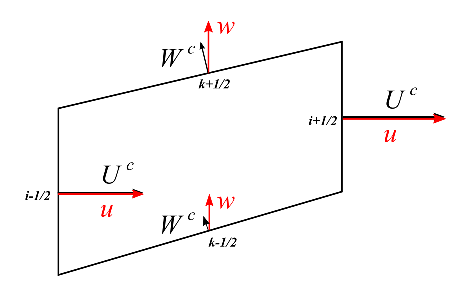
\includegraphics[width=19pc]{\EPSDIR/dessin_contravariant.eps}
	 \caption{Representation of the wind ($u$, $w$) and its contravariant components ($U_c$, $W_c$) on the C-grid in the 2D vertical plane ($x$, $z$).}
 \label{fig:contrav}
\end{figure}

To simplify, we consider only the $x$-momentum equation, and its $x$-derivative term:
\begin{equation}
 \frac{\partial (\tilde{\rho} U^{c} u)}{\partial \overline{x}} = \frac{\partial (F_C(\tilde{\rho} U^{c})F(u))}{\partial \overline{x}}.
 \label{eq:flux-form}
\end{equation}

 $F_C(\tilde{\rho} U^{c})$ contains the topologic terms, which integrate terrain transformations. The second flux $F(u)$ is calculated on the mesh point without considering any terrain transformation, using the advection method. All the other derivative terms are built with a similar methodology.
 
Because of the Arakawa C-grid, the advector (contravariant components) and the transported wind field ($u$, $v$ and $w$) present different directions. 
The discrete form of the contravariant metric terms is of 4$^{th}$ order on the vertical direction, in agreement with Klemp et al. (2003), and of 2$^{nd}$ order on the horizontal directions. 

Defining $i$ as the spatial index in the $x$-direction and $\Delta x$ the mesh step size, the derivative is written so:
\begin{equation}
\begin{split}
 \frac{\partial (\tilde{\rho} U^{c} u)_i}{\partial \overline{x}} =& \frac{F_C(\tilde{\rho} U^{c})_{i+1/2} F(u)_{i+1/2}}{\Delta x} 
 - \frac{F_C(\tilde{\rho} U^{c})_{i-1/2} F(u)_{i-1/2}}{\Delta x}.
 \label{eq:flux-form-num}
\end{split}
\end{equation}

Then, a chosen discretization is applied to the flux terms $F$, following its definition using the flux formulation:
\begin{equation}
	\frac{\partial u_i}{\partial x} = \frac{F(u)_{i+1/2}-F(u)_{i-1/2}}{\Delta x}.
	\label{eq:discr_op}
\end{equation}
Two different methods, each with two distinct orders, can be used to discretize $F$: a WENO discretization of 5$^{th}$ or 3$^{rd}$ order (WENO5 and WENO3, respectively), or a centered discretization of 4$^{th}$ or 2$^{nd}$ order (CEN4TH and CEN2ND, respectively).

\subsection{Discretization with the WENO schemes}
The WENO schemes owe their success to the use of a dynamic set of stencils, where a nonlinear convex combination of lower order polynomials adapts either to a higher order approximation at smooth parts of the solution, or to an upwind spatial discretization that avoids interpolation across discontinuities and provides the necessary dissipation for shock capturing (Jiang and Shu, 1995; Shu, 1998). They allow a better representation of the solution in presence of high 
    gradients. Pressel et al. (2015) have shown the advantages of the WENO schemes from 3$^{rd}$ through 11$^{th}$ order for the transport of scalars and momentum over central difference schemes.

The first step consists on separating the velocity flux terms into positive and negative fluxes, using Lax-Friedrich flux splitting as in Shu (1998):
\begin{equation}
F_{\mbox{WENO}}(u)_{i+1/2} = f^{+}_{i+1/2} + f^{-}_{i+1/2}.
\label{eq:flux-splitting}
\end{equation}
In the following development, only the reconstruction of the positive fluxes is described. The reader can refer to Wang and Spiteri (2007), Shu (1998) and Castro et al. (2011) for a more detailed description. The velocity fluxes are built using a stencil given by a Lagrangian interpolation using the velocity average on each cell.

~\\
For WENO5, the stencil is given by:
\begin{equation}
\begin{split}
 f^+_{i+1/2} =& \; \gamma_0 \left( \dfrac{2}{6} \bar{u}_{i-2} - \dfrac{7}{6} \bar{u}_{i-1} + \dfrac{11}{6} \bar{u}_{i} 
 \right) \\
 &+ \gamma_1 \left(-\dfrac{1}{6} \bar{u}_{i-1} + \dfrac{5}{6} \bar{u}_{i}   + \dfrac{2}{6} \bar{u}_{i+1} \right) \\ 
 &+ \gamma_2 \left( \dfrac{2}{6} \bar{u}_{i}   + \dfrac{5}{6} \bar{u}_{i+1} - \dfrac{1}{6} \bar{u}_{i+2} \right)     
\end{split}    
\end{equation}

with the average value for the velocity defined by:

\begin{equation}
 \bar{u}_i = \dfrac{1}{\Delta x_i} \int_{x_{i-1/2}}^{x_{i+1/2}} u(\xi)d\xi.
\end{equation}

The strength of the WENO5 method relies on the choice of the WENO stencil weights $\gamma_j$. These allow to keep a non-oscillatory solution even in presence of shock or high gradient in the velocity field. They are given by:
\begin{equation}
 \gamma_j = \dfrac{\alpha_j}{\alpha_0+\alpha_1+\alpha_2}
\end{equation}
where the non-normalized stencil weights are:
\begin{equation}
\begin{split}
 \alpha_0 = \dfrac{1}{10} \left( \dfrac{1}{\epsilon + \beta_0} \right) ^2 , \;
 \alpha_1 = \dfrac{6}{10} \left( \dfrac{1}{\epsilon + \beta_1} \right) ^2 , \\
 \alpha_2 = \dfrac{3}{10} \left( \dfrac{1}{\epsilon + \beta_2} \right) ^2.
\end{split} 
\end{equation}

The $\epsilon$ term is here to prevent the denominator to be null (it is set to $10^{-15}$ in the model). The $\beta_j$ terms, also called indicators of smoothness, are the heart of essentially non-oscillatory (ENO) methods, from which the WENO schemes are extended. They are defined as:
\begin{align}
 \beta_0 &= \dfrac{13}{12} \left( \bar{u}_{i-2} - 2\bar{u}_{i-1} + \bar{u}_{i} \right)^2 + \dfrac{1}{4} \left( \bar{u}_{i-2} - 4\bar{u}_{i-1} + 3\bar{u}_{i} \right)^2 \nonumber \\
 \beta_1 &= \dfrac{13}{12} \left( \bar{u}_{i-1} - 2\bar{u}_{i} + \bar{u}_{i+1} \right)^2 + \dfrac{1}{4} \left( \bar{u}_{i-1} - \bar{u}_{i+1} \right)^2 \\
 \beta_2 &= \dfrac{13}{12} \left( \bar{u}_{i} - 2\bar{u}_{i+1} + \bar{u}_{i+2} \right)^2 + \dfrac{1}{4} \left( 3\bar{u}_{i} - 4\bar{u}_{i+1} + \bar{u}_{i+2} \right)^2. \nonumber
\end{align}

WENO5 reverts to WENO3 at the edges of the computational domain for open boundary conditions only.

~\\
For WENO3, the stencil is given by:
\begin{equation}
 f^+_{i+1/2} = \gamma_0 \left(-\dfrac{1}{2} \bar{u}_{i-1} + \dfrac{3}{2} \bar{u}_{i} \right) +
	         \gamma_1 \left(\dfrac{1}{2} \bar{u}_{i} + \dfrac{1}{2} \bar{u}_{i+1} \right).     
\end{equation}
The stencil weights are:
\begin{equation}
 \gamma_j = \dfrac{\alpha_i}{\alpha_0+\alpha_1}
\end{equation}
where the non-normalized stencil weights are:
\begin{equation}
 \alpha_0 = \dfrac{1}{3} \left( \dfrac{1}{\epsilon + \beta_0} \right) ^2 , \;
 \alpha_1 = \dfrac{2}{3} \left( \dfrac{1}{\epsilon + \beta_1} \right) ^2 
\end{equation}
and for the smoothness indicators:
\begin{equation}
 \beta_0 = \left(-\bar{u}_{i-1} + \bar{u}_{i} \right)^2  , \;
 \beta_1 = \left(-\bar{u}_{i} + \bar{u}_{i+1} \right)^2.
\end{equation}

The computational cost of WENO3 is much lower than WENO5, but WENO3 is known to be strongly more diffusive (Tan et al., 2005). The use of explicit numerical diffusion applied to wind fields with WENO schemes is
prohibited. WENO5 requires a halo of 3 points between adjacent processors (NHALO=3).

\subsection{Discretization with centered schemes}

For centered schemes, no flux decomposition is required. The fluxes are directly computed using a 4$^{th}$-order reconstruction for CEN4TH:
\begin{equation}
F_{\mbox{CEN4TH}}(u)_{i+1/2} = \frac{7(u_{i+1}+u_{i})-(u_{i+2}+u_{i-1})}{12}
\end{equation}

or a 2$^{nd}$ order for CEN2ND:
\begin{equation}
F_{\mbox{CEN2ND}}(u)_{i+1/2} = \frac{u_{i+1}+u_{i}}{2}
\end{equation}

CEN4TH reverts to CEN2ND at the edges of the computational domain for open boundary conditions only.

The centered schemes must be also combined with numerical diffusion operator of 4$^{th}$ order in the model, in order to damp numerical energy accumulation in the shortest wavelengths. 
The 4$^{th}$ order centered scheme presents a good accuracy (the effective resolution is of order of 5--6 $\Delta x$; Ricard et al., 2013) and it is easy to implement.

\subsection{Temporal schemes for momentum}

Once the space derivatives are estimated, a temporal discretization is used to integrate the fluxes in time from the current state to the next one. 
A common strategy to improve computational efficiency is to use explicit numerical schemes integrating the high-frequency modes with a small time step and lower-frequency modes with a larger time step.
Wicker and Skamarock (2002) were among the first to use a $3^{rd}$-order explicit Runge-Kutta (ERK) scheme. Higher order time-stepping combinations have been studying since them, especially combined with WENO spatial discretization (e.g. Wang and Spiteri, 2007).

For the WENO schemes employed in Meso-NH, some ERK methods of high order are implemented.
An explicit splitting method can be added to improve a bit more the stability properties as presented below.
For centered momentum schemes, only the Leap-Frog (LF) scheme and one specific centered ERK method are available.

\subsubsection{Explicit RK method}

Explicit Runge-Kutta (ERK) methods can be applied to the momentum transport, together with FIT time integration for the rest of the model (contravariant flux $F_C(\tilde{\rho}U^c)$ among others). The general temporal proceeding for one advection term in Eq.~\eqref{eq:mommesonh1}  will then be described.

Using the anelastic hypothesis ($\frac{\partial \rho}{\partial t} = 0$), we consider the tendency of a variable defined by its time-variation induced by the spatial term in the advection equation, noted $T_u$:
$$ T_u = \tilde{\rho} \frac{\partial u}{\partial t} $$,
which is written in the discrete form using the FIT formulation (with $n$ as the temporal index) as:
\begin{equation}
T_u^{n+1} = \tilde{\rho} \frac{u^{n+1}-u^{n}}{\Delta t}
\label{eq:tendency}
\end{equation}

The contravariant flux $F_C(U^c)$ (the \textquotedblleft advector \textquotedblright\ field) is kept constant along the time step, to satisfy the continuity equation. The ERK method is applied on the following equation:
\begin{equation}
\tilde{\rho} \frac{\partial u}{\partial t} = M(u) + S
\label{eq:semi-discr}
\end{equation}
where $M(u)$ is the discrete term defined in Eq.~\eqref{eq:mommesonh1}, and $S$ represents the other terms of the momentum equation. As the solver pressure is called between the call to the momentum advection and the end of the time-step, the pressure contribution of the previous time step is added to the processes computed since the beginning of the current time step. 

\noindent We consider a general s-stage ERK method defined by its Butcher coefficients:
\begin{displaymath}
\begin{array}{c|cccccc}
c_{1} &   &   &   &   &  & \\ 
c_{2} & a_{21} &   &   &   &   & \\
c_{3} & a_{31} & a_{32} &   &   &   & \\
c_{4} & a_{41} & a_{42} & a_{43} &   &   & \\ 
\vdots & \vdots & \vdots & \vdots & \ddots &    &  \\
c_{s} & a_{s1} & a_{s2} & a_{s3} & \ldots & a_{s,s-1} &  \\
\hline
      & b_{1} & b_{2} & b_{3} & \ldots & b_{s-1} & b_{s} 
\end{array}
\end{displaymath}
The advection tendency follows:

\begin{align} 
u^{n}_{1} &=  u^{n} \nonumber \\ 
u^{n}_{k} &=  u^{n} \; + \; \Delta{t} \; \sum_{j=1}^{k-1} \; a_{k,j} \; \frac{M(u^n_j)+S}{\rho^n} \label{eq:erk}\\ 
T_u^{n+1} &= \sum_{k=1}^{s} \; b_{k} \; \left( M(u^{n}_{k}) + S \right). \nonumber
\end{align}


Adding the advection tendency to get $u^{n+1}$ using Eq.~\eqref{eq:tendency} leads to the classical Runge-Kutta method applied to the momentum equation. The different explicit RK methods considered in Meso-NH are:
\begin{multicols}{2}
    \begin{center}
        ERK with order 1 and 2 steps (RK21) \\
        \begin{tabular}{c|cc}
            0    & & \\
            3/4  & 3/4 & \\
            \hline
            & 0 & 1 \\		
        \end{tabular}
    \end{center}
%    \columnbreak
    \begin{center}
        SSP-RK with order 3 and 3 steps (RK33) \\
        \begin{tabular}{c|ccc}
            0   & & & \\
            1   & 1 & & \\
            1/2 & 1/4  & 1/4 &  \\
            \hline
            & 1/6 & 1/6 & 2/3 \\		
        \end{tabular}
    \end{center}
\end{multicols}

\begin{multicols}{2}
\begin{center}
    ERK with order 3 and 5 steps (RK53) \\
    \begin{tabular}{c|ccccc}
        0    & & & & & \\
        1/7  & 1/7 & & & & \\
        3/16 &  0  & 3/16 &   & & \\
        1/3  &  0  &  0   & 1/3 & & \\
        2/3  &  0  &  0   & 0   & 2/3 & \\
        \hline
        & 1/4 & 0 & 0 & 0 & 3/4 \\		
    \end{tabular}
\end{center}

\begin{center}
    ERK order 4 (RKC4) \\
    \begin{tabular}{c|cccc}
        0   & & & & \\
        1/2 & 1/2 & & & \\
        1/2 &  0  & 1/2 &   & \\
        1   &  0  &  0  & 1 & \\
        \hline
        & 1/6 & 1/3 & 1/3 & 1/6 \\		
    \end{tabular}
\end{center}
\end{multicols}


RK33 requires more memory storage 
than the RKC4 and RK53 methods, as RK33 has a plain Butcher matrix. In contrast, RKC4 and RK53 have a diagonal Butcher matrix, so they only need to store 
one field in memory at each stage to compute the next one, justifying the classification of low-storage ERK methods.
 
\noindent WENO3 and WENO5 can be used with all the ERK schemes presented above.

\noindent CEN4TH can only be used with RKC4, or without RK time splitting with the classical Leap-Frog scheme. CEN2ND can only be used with the Leap-Frog scheme.

\subsubsection{Additional time splitting method}

To increase a bit more the maximum CFL number, an additional time-splitting can be activated for the wind advection with WENO. Considering one time step $[t_n,t_{n+1}]$, we divide it into $L$ regular sub-steps $[t_l,t_{l+1}]$ with $t_n=t_0 < ... < t_l < t_{l+1} < ... < t_L=t_{n+1}$. 

Once one value $u^l$ is known ($u^0$ at first), the next value $u^{l+1}$ is computed using Eq.~\eqref{eq:tendency} with $\Delta t = t_{l+1} - t_l$, that is:
\begin{equation}
T_u^{l+1} = \rho \frac{u^{l+1}-u^{l}}{\Delta t}
\end{equation}
with $u^{l+1}$ computed using all stages of the ERK method as described in Eq.~\eqref{eq:erk}. This process is repeated $L$ times to compute the $L$ tendencies (Fig.~\ref{fig:time}). At the end, we obtain the tendency on the original final time $t_{n+1}$ by calculating the following average:
\begin{equation}
T_u = \frac{1}{L}\sum_{l=1}^{L} T_u^l.
\end{equation}

The main interest of such an additional time splitting is to call the rest of the model (pressure solver, physics, chemistry, ...) less frequently.



%Hence, to summarize the time-marching in Meso-NH, three time steps are effective 
When WENO schemes are applied to momentum transport (Fig.~\ref{fig:time}), the larger time step is applied to all the model components including the physics and the pressure solver, with the FIT temporal scheme. The advection of all variables is conducted with a constant advection momentum vector.
A smaller time step is used for wind advection applying the ERK method on the subinterval. 

\noindent With the centered momentum transport schemes, there is no additional time splitting.
Therefore, when CEN4TH is applied to momentum transport with the RKC4 time marching, there is no sub-step $l$ for momentum. When it is applied with the Leap-Frog scheme, there is neither ERK time-splitting nor sub-step $l$.



\begin{figure}[t]
 \centering
    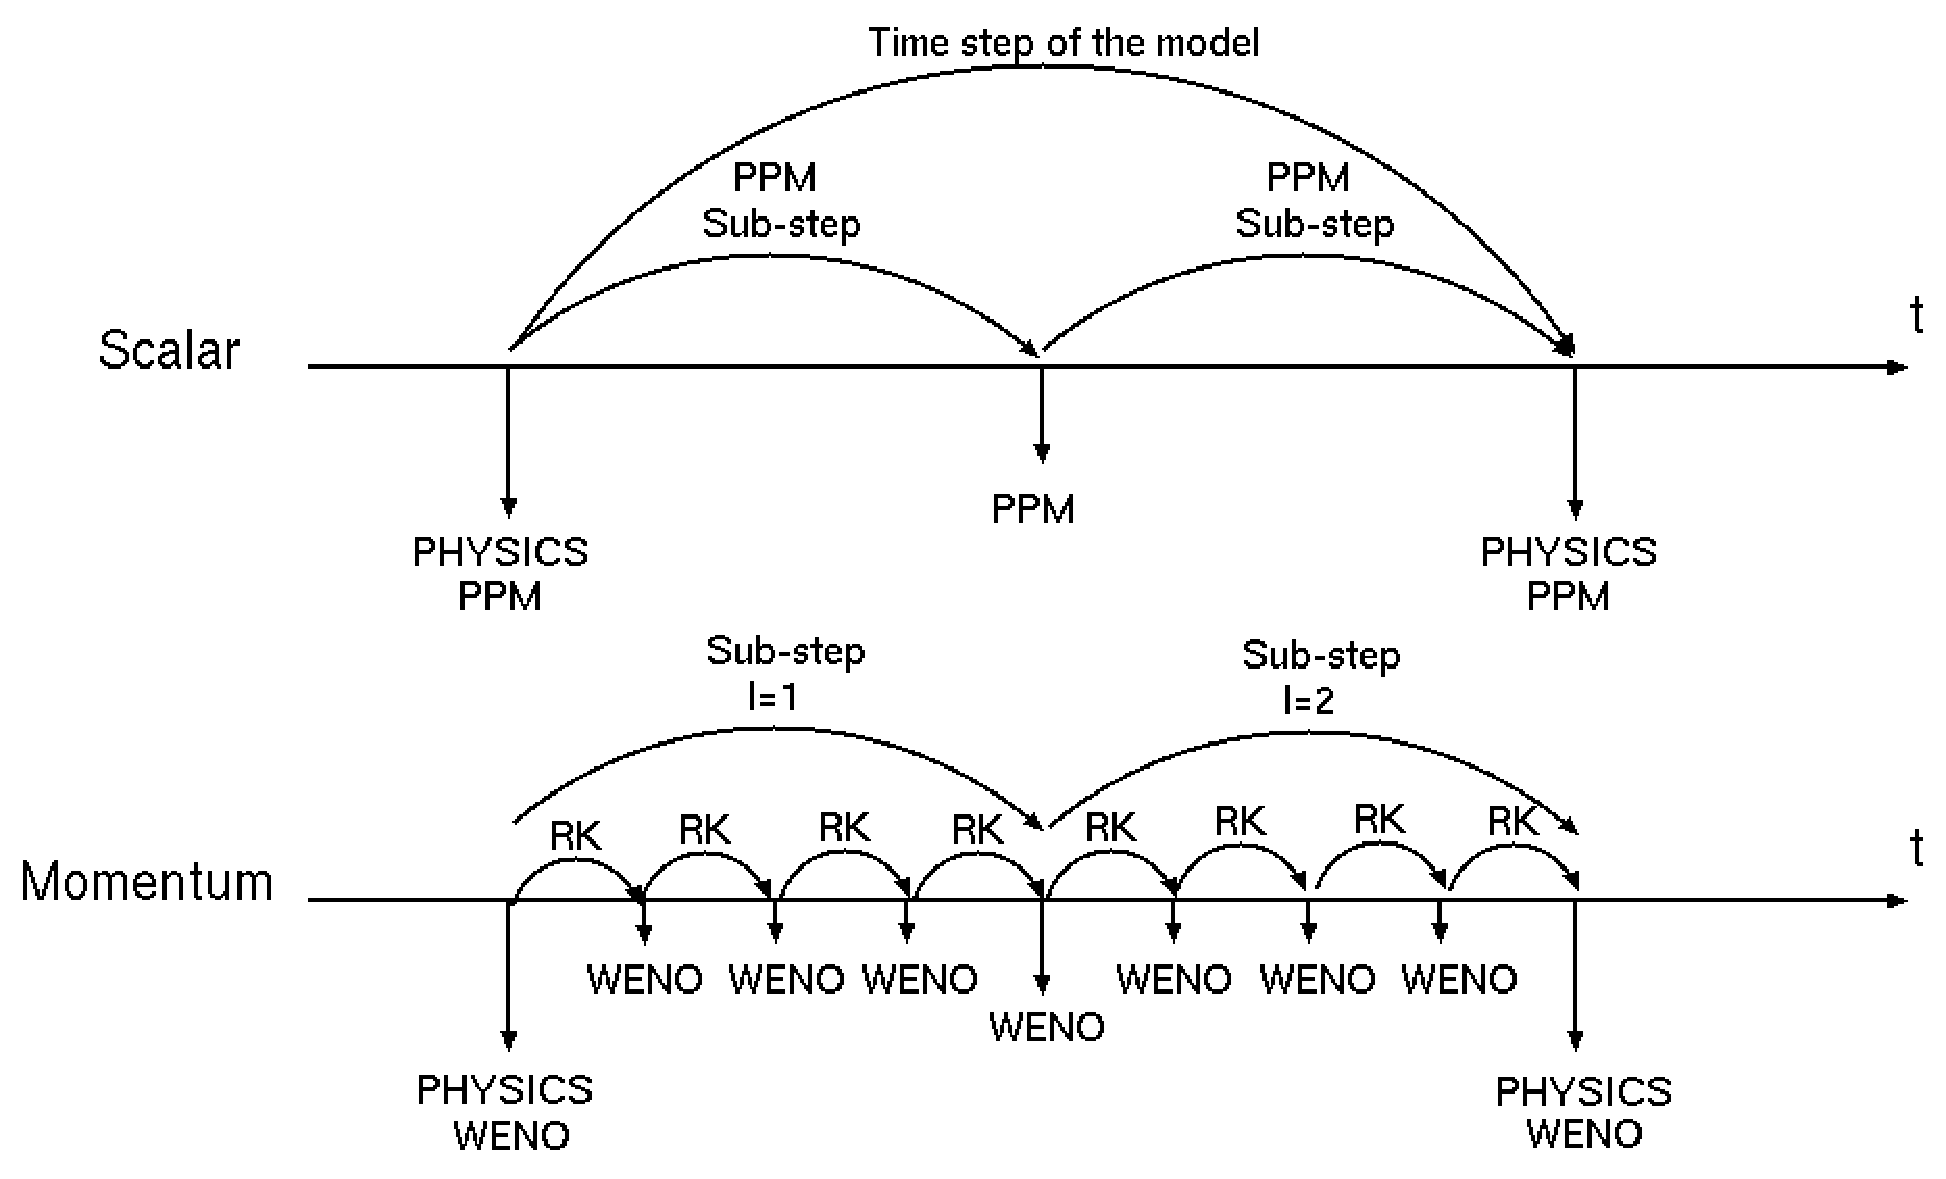
\includegraphics[width=19pc]{\EPSDIR/timescheme.eps}
    \caption{Representation of the time-marching in Meso-NH with WENO schemes for the transport of momentum and scalar variables.}
    \label{fig:time}
\end{figure}


\subsubsection{Comparison on the 2D hydrostatic mountain wave}

A classical evaluation of the momentum advection schemes involves the steady-state solution of linear 2D hydrostatic flow over a single-peaked mountain with constant inflow, as in Durran and Klemp (1983) and Xue and Thorpe (1991). The profile of the symmetric Witch of Agnesi mountain is used as: 
$$ h(x) = h_{\max}\frac{a^2}{x^2 + a^2}$$ with $h_{\max}=1~m$ the height and $a=10$~km the half-width of the mountain. The initial state of the atmosphere consists of a constant mean flow with $U=20$~m~s$^{-1}$, a ground potential temperature of $\theta=250$~K, and a Brunt-Väisälä frequency $N=0.02$~s$^{-1}$. The resolution is  $\Delta x = 500$~m and $\Delta z = 250$~m, and the domain extends horizontally over 800~km and vertically over 30~km. A Rayleigh damping layer is applied above 22~km. Figure~\ref{fig:whydro} shows that the numerical (dashed grey) values of vertical velocity and the analytical (colored contours) ones compare well. The simulation is shown here only for WENO5 as the differences with the various advection schemes are too tiny to be visible.

\begin{figure}[ht]
    \centering
    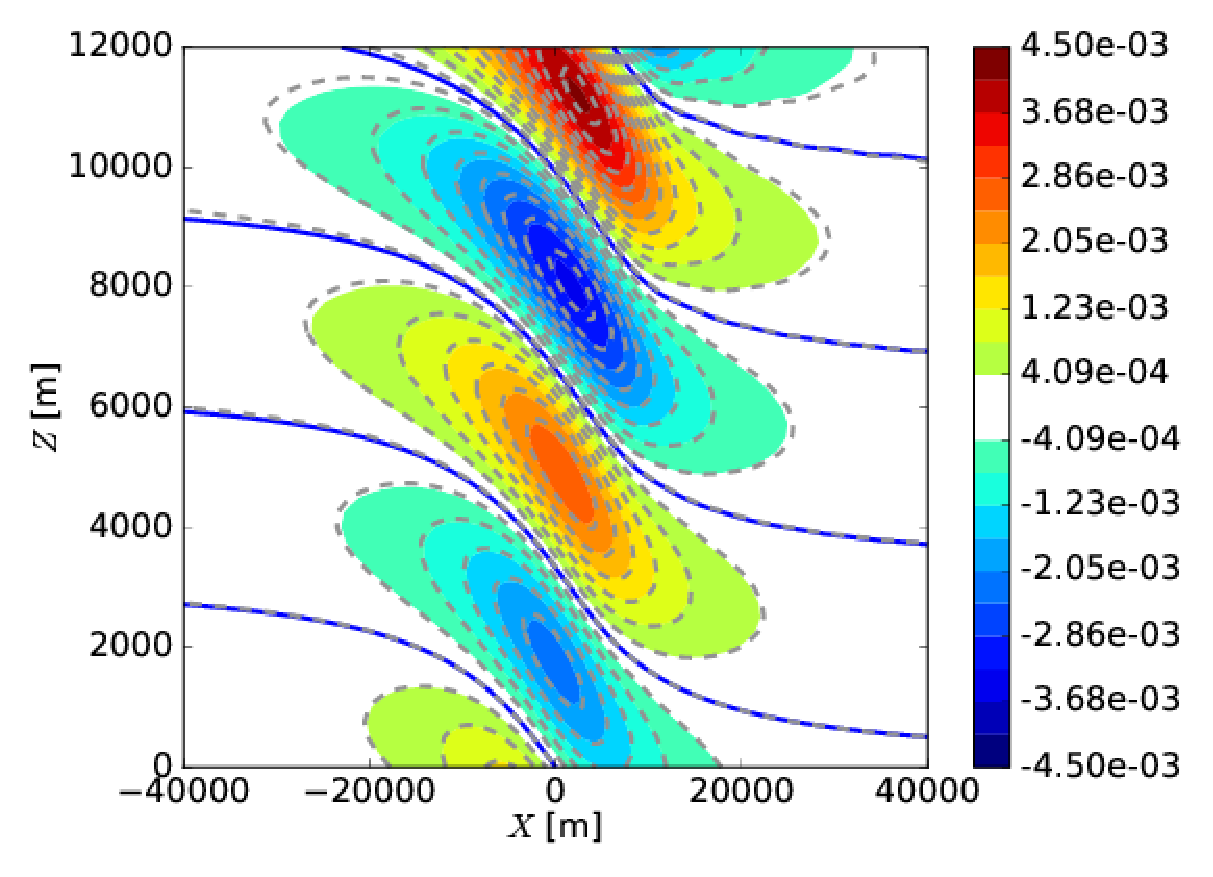
\includegraphics[width=19pc]{\EPSDIR/AGN_H_W5OPE.eps}
    \caption{Case of linear hydrostatic mountain. Vertical cross-section of vertical velocity (m~s$^{-1}$) after 10~h. Colored isovalues correspond to the analytical solution, and dashed grey lines to the numerical one, given here for WENO5 and RK53, with CFL$=0.4$.}
    \label{fig:whydro}
\end{figure}

But there are some significant differences in terms of maximum CFL number and wall clock time to solution.
A stability study, including the additional time-splitting for WENO schemes, is presented in Table~\ref{tab:cflH}. It should be noted that this case does not call any physics: only the dynamical sources are involved.

First, the additional time-splitting for WENO schemes is only presented with $L=2$ as $L=3$ does not improve the maximum CFL number.

Without any additional time-splitting for WENO schemes, the CFL numbers are maximum for CEN4TH/RKC4, and WENO5/WENO3 combined with RKC4/RK53. In contrast, the lowest CFL number is given by CEN4TH/LF.
RK33 gives a maximum CFL number lower than RK53 and RKC4 with the WENO schemes (it requires more memory storage as explained above). 

\noindent The computational cost is significantly lower with CEN4TH/RKC4, while WENO5 requires strong computational effort. WENO3/RKC4 costs almost the same than CEN4TH/RKC4 at equal CFL number. Lastly, RKC4 and RK53 produce equivalent maximum CFL numbers with WENO schemes, but RKC4 is slightly cheaper with 4 stages instead of 5 for RK53.

With additional time-splitting for the WENO schemes, the maximum CFL number is significantly increased with RKC4/RK53 methods, up to 1.8 with WENO5 and 2.5 with WENO3. The impact is not obvious on the wall clock time to solution, because this case only involves dynamical processes. But it will be more significant on cases with physics, and even more with chemistry.



\begin{table}[ht]
\centering
\begin{tabular}{ l c c c c c c}
\hline\hline
       &  LF  &  RK33 & RK53 & RKC4 \\
\hline
CEN4TH & 0.4 &  &  &  1.5 \\
& \it{1} &  &  & \it{0.42} \\
\hline
WENO-3 &  &  &  &  \\
L=1 &  & 1.0 & 1.3 & 1.3 \\
&  & \it{0.74} & \it{0.63} & \it{0.58} \\
L=2 &  & 2.1 & 2.5 & 2.5 \\
&  & \it{0.52} & \it{0.57} & \it{0.54} \\
\hline
WENO-5 &  &  &  &  \\
L=1 &  & 1.0 & 1.4 & 1.4 \\
&  & \it{2.15} & \it{1.95} & \it{1.76} \\
L=2 &  & 1.7 & 1.8 & 1.8 \\
&  & \it{1.99} & \it{2.51} & \it{2.21} \\
\hline

\end{tabular}
\caption{Case of linear hydrostatic flow for CEN4TH and for WENO schemes combined with ERK methods and additional time-splitting ($L$ is the split number): maximum CFL number and computational cost for the maximum CFL number in italics to run 15000 s, considering the computational cost of CEN4TH/LF as the unit.}
\label{tab:cflH}
\end{table}


\subsubsection{Recommendations}



Other tests have shown that:
\begin{itemize}
\item CEN4TH/RKC4 presents the best effective resolution, and the less diffusive behaviour, followed by CEN4TH/LF and then WENO5/RK53-RKC4. This is crucial for LES of clouds: the entrainment of environmental at the cloud edges is higher with CEN4TH/RKC4 as the implicit diffusion is lower. 
 \item WENO3 is excessively damping and is prohibited for LES as the effective resolution is of the order of $12 \Delta x$.
 \item WENO5/RK53-RKC4 is well adapted to sharp gradients area, i.e. in complex shock-obstacle interactions with immersed boundary method. 
 \item CEN4TH/LF is much more expensive than CEN4TH/RKC4
\end{itemize}

Therefore the recommendations could be:
\begin{itemize}
 \item CEN4TH/RKC4 is recommended for LES.
 \item WENO5/RKC4 is recommended for simulations with expensive chemistry/physics, typically mesoscale simulations, or for simulations with sharp-gradient area.
\end{itemize}






\section{Advection schemes for scalar variables: the PPM}

\subsection{Introduction}

  The PPM advection scheme is based on the piecewise
  parabolic method (PPM), a numerical technique developed in
  astrophysics for modeling fluid flows (Colella et al.\ 1984, Carpenter
  et al.\ 1990). The PPM scheme differs substantially from conventional
  grid-point methods like the 2$^{nd}$- and 4$^{th}$-order centered advection
  schemes. It is a finite-volume
  method in which some assumption is made about the structure of the
  approximate solution between the grid points. In the PPM case,
  piecewise continuous parabolas are fitted in each grid-cell. This
  design enables the scheme to handle sharp gradients and
  discontinuities very accurately. Although the constructed piecewise
  continuous functions would allow for the explicit calculation of
  derivatives, in practice the advective forcing is computed from the
  fluxes at the grid-cell edges. Various flux limiters can be used to
  ensure the scheme is monotonic. Monotonic schemes do not amplify
  extrema in the initial values and are, thus, also positive
  definite. Application of the PPM schemes to 3D problems requires
  density-corrected directional splitting and FIT time-marching.

  Three different versions of the PPM advection scheme have been
  implemented in Meso-NH: the unrestricted scheme PPM\_00 and two monotonic
  versions, PPM\_01 and PPM\_02. PPM\_01 is based on the original scheme (Colella at al.\ 1984)
  with monotonicity constraints modified by Lin and Rood (1996) while
  PPM\_02 uses the flux limiter developed by Skamarock (2006).
  PPM\_02 permits extension to stable semi-Lagrangian integrations
  using CFL numbers larger than one. 
  The PPM schemes are intended for advection of meteorological
  variables (e.g.\ temperature, water species, TKE) and passive
  scalars. All three versions have excellent mass-conservation properties
  and were found to be an order of magnitude more accurate than the
  centered 4\ts{th} order (CEN4TH) scheme previously applied to scalar variables in idealized
  2D tests. However, the implicit numerical diffusion associated with the
  monotonicity preserving methods in PPM\_01 and PPM\_02 can damp
  smooth, well resolved extrema. Therefore the use of explicit numerical diffusion
  applied to scalar fields should be prohibited when using the PPM schemes.
  Also, the flux limiters and the
  specific time marching require computational effort
  making the monotonic PPM schemes significantly more expensive than a classical centered scheme. 

  \subsection{Description}

  The advective part of the scalar conservation equation can be written
  as:  
  \begin{equation}
    \label{advection}
    \frac{\pl}{\pl t}(\tilde{\rho} \phi) =
    - \frac{\pl}{\pl x}(\tilde{\rho} U_c \phi)
    - \frac{\pl}{\pl y}(\tilde{\rho} V_c \phi)
    - \frac{\pl}{\pl z}(\tilde{\rho} W_c \phi)    
  \end{equation}
  where in the same way as for the transport of wind, the contravariant components of the wind field are the \textquotedblleft advector \textquotedblright field $(U_c,V_c,W_c)$. To simplify the notation, we will consider in the following part $(u,v,w)$ instead of $(U_c,V_c,W_c)$, as if we were in a Cartesian framework. To solve this
  equation on a discrete grid using the PPM finite-volume method, an
  approximate solution for the scalar field $\phi$ is constructed
  between the grid points. The grid-point value $\phi_{i}$ of a scalar
  variable at a mass grid point $i$ represents the average of the
  function $\phi(x)$ over the grid-cell, or the interval $x_{i-1/2} \le
  x \le x_{i+1/2}$, where the $x_{i-1/2}$ and $x_{1+1/2}$ are the
  neighboring momentum grid points. In the PPM case, the function
  $\phi(x)$ is a parabola which is constructed uniquely for each
  grid-cell using the cell mean ($\phi_{i}$) and values at the cell
  edges ($\phi_{i-1/2}$ and $\phi_{i+1/2}$).  Once the parabolas are
  known, we can calculate fluxes at the grid-cell edges, and the net
  scalar transport in each cell is equal to the flux divergences.

  A solution (in one dimension) to Eq.~(\ref{advection}) can be calculated
  from the FIT discretization:
  \begin{equation}
    \label{1DFIT}
    (\tilde{\rho} \phi)_{i}^{t+\Delta t} = (\tilde{\rho} \phi)_{i}^{t} -
    \mathcal{F}_{x,i}(\phi^{t})    
  \end{equation}
  where the operator $\mathcal{F}_{x,i}$ denotes the discrete flux
  divergence in the grid-cell $i$ and is expressed as:
  \begin{equation}
    \label{FIT}
    \mathcal{F}_{x,i}(\phi^{t}) = \frac{\Delta t}{\Delta x_{i}} \left[
      (\tilde{\rho} u)_{i+1/2} f(\phi^{t})_{i+1/2} - (\tilde{\rho} u)_{i-1/2}
      f(\phi^{t})_{i-1/2} \right] 
  \end{equation}
  where $F_{i\pm1/2}=(\tilde{\rho} u)_{i\pm1/2} f(\phi^{t})_{i\pm1/2}$ are the
  scalar fluxes at the grid-cell edges. These fluxes can be determined
  by integrating over the parabolas in each cell. The parabola in the
  grid-cell $i$ (dropping the superscript $t$) is constructed from the
  cell average ($\phi_{i}$) and left- and right-edge values ($\phi_{L,i}$
  and $\phi_{R,i}$) in the following way:
  \begin{equation}
    \label{par}
    \phi_{i}(\xi) = \phi_{L,i} + \xi \left[ \Delta(\phi)_{i} +
      \phi_{6,i} \left ( 1- \xi \right ) \right ], \quad \xi = \frac{x -
      x_{i-1/2}}{\Delta x_{i}}
  \end{equation}
  where $0 \le \xi \le 1$ ($x_{i-1/2} \le x \le x_{i+1/2}$) is the
  horizontal coordinate. The parameters of the parabola are:
  \begin{eqnarray}
    \Delta(\phi)_{i} & = & \phi_{R,i} - \phi_{L,i}\\
    \phi_{6,i} & = & 6 \left[\phi_{i} - \frac{1}{2}\left (\phi_{R,i} +
    \phi_{L,i} \right ) \right ].
  \end{eqnarray}
  The edge values are determined using the 4\ts{th} order differencing:
  \begin{eqnarray}
    \label{edgevalues1}
    \phi_{L,i} &=& \phi_{i-1/2} = \frac{1}{2}\left ( \phi_{i} + \phi_{i-1}
    \right ) - \frac{1}{6}\left ( \delta(\phi_{i}) - \delta(\phi_{i-1})
    \right )\\
    \label{edgevalues2}
    \phi_{R,i} &=& \phi_{i+1/2} = \frac{1}{2}\left ( \phi_{i+1} + \phi_{i}
    \right ) - \frac{1}{6}\left ( \delta(\phi_{i+1}) - \delta(\phi_{i})
    \right )
  \end{eqnarray}
  where the operator $\delta(\,)$ is defined as:
  \begin{equation}
    \label{endpar}
    \delta(\phi_{i}) = \frac{1}{2} \left( \phi_{i+1} - \phi_{i-1} \right).
  \end{equation}  
  Finally, the scalar fluxes at the edges of grid-cells
  ($f(\phi)_{i\pm1/2}$) are calculated as the average value of the scalar
  over the advective distance in each grid cell:  
  \begin{equation}
    f(\phi)_{i+1/2} = \frac{1}{\Delta t u_{i+1/2}}
    \int_{x_{i+1/2}-\Delta tu_{i+1/2}}^{x_{i+1/2}} \phi_{i}(x) \dif x,
    \quad \mathrm{for} \quad u_{i+1/2} > 0
  \end{equation}
  Substituting Eqs.~(\ref{par}) through (\ref{endpar}) we get:
  \begin{equation}
    \label{flux+}
    f(\phi)_{i+1/2}^{+} = \phi_{R,i} -
     \frac{1}{2} Cr_{i+1/2} \left[\Delta(\phi)_{i} - 
     \left(1- \frac{2}{3} Cr_{i+1/2} \right) \phi_{6,i} \right]
  \end{equation}
  for $Cr_{i+1/2} \geq 0$,
  \begin{equation}
    \label{flux-}
    f(\phi)_{i+1/2}^{-} = \phi_{L,i+1} -
     \frac{1}{2} Cr_{i+1/2} \left[ \Delta(\phi)_{i+1} + 
     \left(1 + \frac{2}{3} Cr_{i+1/2} \right) \phi_{6,i+1} \right]
  \end{equation}
  for $Cr_{i+1/2} < 0$. Here $Cr_{i+1/2} = u_{i+1/2}\Delta t/\Delta x$
  is the CFL number. 

  \subsubsection{The PPM\_00 unrestricted scheme}

  The PPM advective fluxes $f_{i\pm1/2}$ can be expressed in a more
  concise way for more efficient calculation. Combining Eqs~(\ref{par})
  through (\ref{endpar}) with the expressions for the fluxes
  [Eqs.~(\ref{flux+}),(\ref{flux-})], we get:
  \begin{eqnarray}
    \label{sflux+}
    f(\phi)_{i+1/2}^{+} &=& \phi_{i+1/2} - Cr_{i+1/2}(\phi_{1+1/2} -
    \phi_{i}) \\ \nonumber
    & & - Cr_{i+1/2}(1-Cr_{i+1/2})(\phi_{i-1/2} - 2\phi_{i} +
    \phi_{i+1/2})    
  \end{eqnarray}
  for $Cr_{i+1/2} = u_{i+1/2}\Delta t/\Delta x \geq 0$,
  \begin{eqnarray}
    \label{sflux-}
    f(\phi)_{i+1/2}^{-} &=& \phi_{i+1/2} + Cr_{i+1/2}(\phi_{1+1/2} -
    \phi_{i+1}) \\ \nonumber
    & & + Cr_{i+1/2}(1+Cr_{i+1/2})(\phi_{i+1/2} - 2\phi_{i+1} +
     \phi_{i+3/2}) 
  \end{eqnarray}
  for $Cr_{i+1/2} = u_{i+1/2}\Delta t/\Delta x < 0$. The values at the
  grid-cell edges (from Eqs.~(\ref{edgevalues1}) and
  (\ref{edgevalues2})) can be expressed as:
  \begin{equation}
    \label{sedgevalues}
    \phi_{i+1/2} = \left [7(\phi_{i+1} + \phi_{i}) - (\phi_{i+2} +
     \phi_{i-1}) \right ]/12.
  \end{equation}
    
  \subsubsection{The PPM\_01 monotonic scheme}  

  When sharp gradients or discontinuities are present in the scalar
  field, the piecewise continuous parabolas can have very steep
  gradients and produce non-physical values -- overshoots
  (e.g. concentrations higher than 100 \%) or undershoots (e.g. negative
  concentrations) somewhere inside the grid-cell. In those cases the
  calculated advective forcing (given by cell-edge fluxes (Eqs.~\ref{flux+})
  and (\ref{flux-})) would likely result in non-physical values in the
  scalar field after the advection step. To avoid the introduction of
  new extrema (overshoots or undershoots) in the domain, monotonicity
  constraints can be imposed on the advection scheme. In the PPM case,
  this can be achieved in two ways: modifying the parabolas or limiting
  the cell-edge fluxes.

  In the original PPM scheme (Colella 1984) the monotonicity is ensured
  by modifying the parameters of the parabolas. Lin and Rood (1996) have
  proposed simplified monotonicity constraints that require fewer
  floating-point operations. The parabola parameters $\delta(\phi_{i})$,
  $\Delta(\phi)_{i}$, $\phi_{6,i}$, $\phi_{L,i}$ and $\phi_{R,i}$ are
  modified in the following way. The average slope $\delta(\phi_{i})$ in
  the $i^{\mathrm{th}}$ grid-cell is replaced by the modified version
  $\delta_{m}(\phi_{i})$:  
  \begin{eqnarray}
    \delta_{m}(\phi_{i}) &=& \mathrm{sign}(\delta(\phi_{i})) \times \\
    \nonumber
    & & \min \left [ |\delta(\phi_{i}) |, \,
      2(\phi_{i}-\phi^{\mathrm{min}}_{i}), \, 2(\phi^{\mathrm{max}}_{i} -
    \phi_{i}) \right ] \\    \nonumber
    \phi^{\mathrm{min}}_{i}&=& \min (\phi_{i-1}, \phi_{i},
    \phi_{i+1}) \\ \nonumber
    \phi^{\mathrm{max}}_{i} &=& \max (\phi_{i-1}, \phi_{i}, \phi_{i+1})
  \end{eqnarray}
  The first-guess parabola coefficients ($\Delta(\phi)_{i}$,
  $\phi_{6,i}$, $\phi_{L,i}$, $\phi_{R,i}$) are calculated using the
  modified $\delta_{m}(\phi_{i})$. The parameters are then adjusted to
  eliminate overshoots and undershoots through the following algorithm:
  \begin{description}
    \label{ppm01}
    \item \texttt{IF} \hspace{5mm} $\delta_{m}(\phi_{i}) = 0$ \\       
       $\hat{\phi}_{L,i} = \phi_{i}, \qquad \hat{\phi}_{R,i} = \phi_{i}, \qquad
       \hat{\phi}_{6,i} = 0$
    \item \texttt{ELSE IF} \hspace{5mm} $\phi_{6,i} \Delta(\phi)_{i} <
      -(\Delta(\phi)_{i})^{2}$ \\
       $\hat{\phi}_{6,i} = 3(\phi_{L,i} - \phi_{i}), \qquad \hat{\phi}_{R,i} =
       \phi_{L,i} - \hat{\phi}_{6,i}, \qquad \hat{\phi}_{L,i} = \phi_{L,i}$
    \item \texttt{ELSE IF} \hspace{5mm} $\phi_{6,i} \Delta(\phi)_{i} >
      (\Delta(\phi)_{i})^{2}$ \\
       $\hat{\phi}_{6,i} = 3(\phi_{R,i} - \phi_{i}), \qquad \hat{\phi}_{L,i} =
       \phi_{R,i} - \hat{\phi}_{6,i}, \qquad \hat{\phi}_{R,i} =
       \phi_{R,i}$
    \item \texttt{END IF}
  \end{description}
  The parameters of the monotonized parabolas (labeled with
  $\hat{\,}\,$) are used to calculate the advective fluxes defined in
  Eqs.~(\ref{flux+}) and (\ref{flux-}).

  \subsubsection{The PPM\_02 monotonic scheme}  

  An alternative way of ensuring monotonicity is by correcting the
  cell-edge fluxes as in the standard FCT approach. This limiter is
  based on the work of Skamarock (2006) and Blossey and Durran
  (2008). The flux at the cell-edge is composed of a
  monotonicity-preserving upwind flux
  \begin{equation}
    F^{\mathrm{up}}_{i+1/2} = \left\{ \begin{array}{ll}
    (\tilde{\rho} u)_{i+1/2} \phi^{t}_{i}, & \mathrm{for} \quad (\tilde{\rho} u)_{i+1/2}
    \ge 0 \\
    (\tilde{\rho} u)_{i+1/2} \phi^{t}_{i+1}, & \mathrm{otherwise} 
    \end{array}\right.
  \end{equation}
  and a higher order correction such that
  \begin{equation}
    F^{m}_{i+1/2} = F^{\mathrm{up}}_{i+1/2} + r_{i+1/2}F^{\mathrm{cor}}_{i+1/2}
  \end{equation}
  where $0 \le r_{i+1/2} \le 1$ and $F^{\mathrm{cor}}_{i+1/2} =
  F^{\mathrm{ppm}}_{i+1/2} - F^{\mathrm{up}}_{i+1/2}$ is the difference
  between the PPM flux (calculated using Eqs.~(\ref{sflux+}) or
  (\ref{sflux-})) and the upstream flux. The resulting flux
  $F^{m}_{i+1/2}$ will produce a monotonic solution in the advection step.

  To evaluate $r_{i+1/2}$ we first calculate an approximate
  ``transported and diffused'' solution using the upwind flux
  \begin{equation}
    (\tilde{\rho} \phi)^{td}_{i} = (\tilde{\rho} \phi)^{t}_{i} - \frac{\Delta t}{\Delta
      x_{i}} \left (F^{up}_{i+1/2} - F^{up}_{i-1/2} \right )
  \end{equation}
  The sum of the correction fluxes directed out of the cell $i$ is
  computed as $F^{\mathrm{out}}_{i} = \max(F^{\mathrm{cor}}_{i+1/2},\, 0) -
  \min(F^{\mathrm{cor}}_{i-1/2},\, 0)$, and the sum of the fluxes
  directed into the cell $i+1$ is calculated as $F^{\mathrm{in}}_{i+1} =
  \max(F^{\mathrm{cor}}_{i+1/2},\, 0) - \min(F^{\mathrm{cor}}_{i+3/2},\,
  0)$. Finally, let
  \begin{equation}
    \phi^{\max,\min}_{i} = \max, \min(\phi^{t}_{i-1}, \, \phi^{t}_{i},
    \, \phi^{t}_{i+1}, \, \phi^{td}_{i-1}, \, \phi^{td}_{i},
    \, \phi^{td}_{i+1})
  \end{equation}
  The re-normalization factor for monotonicity preservation is defined
  as:
  \begin{equation}
    r_{i+1/2} = \max \left [0, \, \min \left(1, \, \frac{[(\tilde{\rho}
          \phi)_{i}^{td} - \hat{\tilde{\rho}}_{i}\phi_{i}^{\min} ]
          \Delta x_{i}}{\Delta t F^{\mathrm{out}}_{i} + \varepsilon}, \,
        \frac{[\hat{\tilde{\rho}}_{i+1} \phi^{\max}_{i+1} - (\tilde{\rho}
          \phi)_{i+1}^{td}] \Delta x_{i+1}}{\Delta t
          F^{\mathrm{in}}_{i+1} + \varepsilon} \right ) \right ]
  \end{equation}
  for $F^{\mathrm{cor}}_{i+1/2} \ge 0$,
  \begin{equation}
    r_{i+1/2} = \max \left [0, \, \min \left(1, \, \frac{[\hat{\tilde{\rho}}_{i}
          \phi^{\max}_{i} - (\tilde{\rho} \phi)_{i}^{td}] \Delta x_{i}}{\Delta t
          F^{\mathrm{in}}_{i} + \varepsilon}, \, \frac{[(\tilde{\rho}
          \phi)_{i+1}^{td} - \hat{\tilde{\rho}}_{i+1}\phi_{i+1}^{\min}
          ] \Delta x_{i+1}}{\Delta t F^{\mathrm{out}}_{i+1} +
          \varepsilon}  \right ) \right ]
  \end{equation}
  for $F^{\mathrm{cor}}_{i+1/2} < 0$. Here $\varepsilon$ is a small
  parameter chosen to avoid division by zero, and $\hat{\tilde{\rho}}$ is the
  density as updated in the current advection step. More details about
  the density correction associated with directional splitting in 3D
  applications will be discussed later. In the final step the cell
  averages are updated to time $t+\Delta t$
  \begin{equation}
    (\tilde{\rho} \phi)^{t+\Delta t}_{i} = (\tilde{\rho} \phi)^{td}_{i} -
    \frac{\Delta t}{\Delta x_{i}} \left
      (r_{i+1/2}F^{\mathrm{cor}}_{i+1/2} -
      r_{i-1/2}F^{\mathrm{cor}}_{i-1/2} \right ).
  \end{equation}

  The PPM\_{02} scheme described here is fully monotonic. It can be
  modified to use semi-Lagrangian approximation to the flux divergence.
  This would extend the domain of dependence beyond the adjacent upstream
  grid-cell and allow stable computation for CFL numbers greater
  than unity. More details about the semi-Lagrangian extension can be
  found in e.g. Skamarock (2006) and Blossey and Durran (2008). For
  Eulerian integration with CFL number less than unity, the PPM\_01 scheme
  is more computationally efficient.

  \subsubsection{Time marching and extension to three dimensions}

  To extend the 1D scalar advection scheme [Eq.~(\ref{1DFIT})] to multiple
  dimensions, we follow the formulation of Easter (1993) where the mass
  conservation $\pl\tilde{\rho}/\pl t + \nabla \cdot (\tilde{\rho} \bvec{V})=0$ is
  simultaneously integrated with the discrete version of the scalar
  transport [Eq.~(\ref{1DFIT})]. This sort of density correction procedure is
  necessary with the PPM schemes because the mass flux ($\tilde{\rho} U$) must
  be saved and updated for scalar advection at each grid-cell
  interface. The density correction is restricted to advection step at time $t+\Delta t$
  and the model overall still uses the selected anelastic
  approximation. The mass conservation is discretized within a 3D
  formulation as:
  \begin{equation}
   \label{mass}
    \tilde{\rho}^{t+\Delta t} = \tilde{\rho}^{t} - \mathcal{F}_{x}(I) -
    \mathcal{F}_{y}(I) - \mathcal{F}_{z}(I),
  \end{equation}
  where the vector $I \equiv 1$ and $\mathcal{F}_{x,y,z}$ denotes the
  discrete flux divergence in $x$, $y$ and $x$ directions, which is
  calculated using the non-monotonic PPM\_00 scheme. The full 3D
  algorithm for simultaneous transport of the scalar and mass
  conservation is:
  \begin{eqnarray}
   \label{easter}
   (\tilde{\rho}\phi)^{*} &=& (\tilde{\rho} \phi)^{t} - \mathcal{F}_{x}(\phi^{t}) \\
   \nonumber
   \tilde{\rho}^{*} &=& \tilde{\rho}^{t} - \mathcal{F}_{x}(I) \\ \nonumber
   \phi^{*} &=& (\tilde{\rho}\phi)^{*} / \tilde{\rho}^{*} \\ \nonumber
   (\tilde{\rho}\phi)^{**} &=& (\tilde{\rho} \phi)^{*} - \mathcal{F}_{y}(\phi^{*}) \\
   \nonumber
   \tilde{\rho}^{**} &=& \tilde{\rho}^{*} - \mathcal{F}_{y}(I) \\ \nonumber
   \phi^{**} &=& (\tilde{\rho}\phi)^{**} / \tilde{\rho}^{**} \\ \nonumber
   (\tilde{\rho}\phi)^{t+\Delta t} &=& (\tilde{\rho} \phi)^{**} -
   \mathcal{F}_{z}(\phi^{**}) \\ \nonumber
   \tilde{\rho}^{t+\Delta t} &=& \tilde{\rho}^{**} - \mathcal{F}_{z}(I) \\ \nonumber
   \phi^{t+\Delta t} &=& (\tilde{\rho}\phi)^{t+\Delta t} / \tilde{\rho}^{t+\Delta t}.
  \end{eqnarray}
  Here the flux-divergence operators $\mathcal{F}_{x,y,z}$ can be
  estimated using any of the described PPM schemes (PPM\_00, PPM\_01 or
  PPM\_02), however the density corrections are always calculated using
  the non-monotonic scheme. The PPM\_00 scheme is the most computationally
  efficient and accuracy of the correction is sufficient even for the
  advection of scalars with the monotonic schemes. 

  It can easily be seen that Eq.~(\ref{easter}) collapses to Eq.~(\ref{mass}) for
  $\phi = I$ and it is consistent (if $\phi$ is constant at initial time
  it remains constant). To achieve 2$^{nd}$-order accuracy of the
  time-split scheme [Eq.~(\ref{easter})] a form of Strang splitting (Strang
  1968) is used. It consists of alternating the order of flux divergence
  operators between $x \rightarrow y \rightarrow z$ to $z \rightarrow y
  \rightarrow x$ at each time step.

  PPM is a finite-volume method and the cell-edge fluxes estimated at
  the current model time $t$ can only be used to calculate the scalar
  values at time $t+\Delta t$ and hence it intrinsically works with
  FIT time-marching. 
  
    \subsubsection{Additional time splitting method}

To increase a bit more the maximum CFL number, an additional time-splitting can be activated  for the scalar advection ($LSPLIT\_CFL$), in order to increase the time step of the rest of the model and to follow a CFL strictly less than 1 for PPM (a threshold of $XSPLIT\_CFL=0.8$ is proposed) (Fig.~\ref{fig:time}). This smaller time step for PPM can evolve during the run as a function of the CFL number.


\bibliographystyle{ametsoc2014}
\bibliography{biblio.bib}

\section{References}
\decrefname
Blossey, P. N. and D. R. Durran, 2008: Selective Monotonicity
   Preservation in Scalar Advection, 
   {\it J. Comput. Phys.},  {\bf 227}, 5160–-5183. 
\decrefname
Carpenter, R. L., K. K. Droegemeier,
   P. R. Woodward, and C. E. Hane, 1990: Application of the
   Piecewise Parabolic Method (PPM) to Meteorological Modeling,
  {\it Mon. Wea. Rev.},  {\bf 118}, 586--612.
\decrefname
Castro, M., B. Costa, and W. S., Don, 2011: High order weighted
   essentially non-oscillatory WENO-Z schemes for hyperbolic conservation laws,
   {\it J. Comput. Phys.},  {\bf 230}, 1766–-1792. 
\decrefname
Colella, P. and P. R. Woodward, 1984: The
   Piecewise Parabolic Method (PPM) for Gas-Dynamical Simulations,
   {\it J. Comput. Phys.},  {\bf 54}, 174--201.
\decrefname
Durran, D. R., and J. B. Klemp, 1983: A compressible model for
   the simulation of moist mountain waves,
   {\it Mon. Wea. Rev.},  {\bf 111 (12)}, 2341-–2361.
\decrefname
Easter, R. C., 1993: Two Modified Versions of Bott's Positive-Definite
   Numerical Advection Scheme, {\it Mon. Wea. Rev.},  {\bf 121}, 297--304.
\decrefname
Gal-Chen, T., and R. C. Somerville, 1975: On the use of a coordinate transformation for the
solution of the Navier-Stokes equations. {\it J. Comput. Phys.},  {\bf 17 (2)}, 209-–228.
\decrefname
Klemp, J. B., W. C. Skamarock, and O. Fuhrer, 2003: Numerical consistency of metric terms in
terrain-following coordinates. {\it Mon. Wea. Rev.}, {\bf 131 (7)}, 1229-–1239.
\decrefname
Jiang, G.-S., and C.-W. Shu, 1995: Efficient implementation of weighted ENO schemes. Tech. rep.,
DTIC Document.
\decrefname
Lin, S. and R. B. Rood, 1996: Multidimensional Flux-Form
   Semi-Lagrangian Transport Schemes, 
   {\it Mon. Wea. Rev.}, {\bf 124}, 2046--2070.
\decrefname
Pressel, K. G., C. M. Kaul, T. Schneider, Z. Tan, and S. Mishra, 2015:
   Large-eddy simulation in an anelastic framework with closed water and entropy
   balances. {\it J. Adv. Model. Earth Syst.}, {\bf 7 (3)}, 1425-–1456.
\decrefname
Ricard, D., C. Lac, S. Riette, R. Legrand, and A. Mary, 2013: Kinetic energy spectra characteristics
of two convection-permitting limited-area models AROME and Meso-NH. {\it Quart. J. Roy. Meteor. Soc.}, {\bf
139 (674)}, 1327-–1341.
\decrefname
Rood, R. B., 1987: Numerical advection algorithms and their role in
   atmospheric transport and chemistry models.
   {\it Rev. Geophys.}, {\bf 25}, 71--100.
\decrefname
Sch\"ar, C., D. Leuenberger, O. Fuhrer, D. L\"uthi, and C. Girard, 2002: A new terrain-following
vertical coordinate formulation for atmospheric prediction models. {\it Mon. Wea. Rev.}, {\bf
130 (10)}, 2459-–2480.
\decrefname
Shu, C.-W., 1998: Essentially non-oscillatory and weighted essentially non-oscillatory schemes
for hyperbolic conservation laws, in Advanced Numerical Approximation of Nonlinear Hyperbolic Equations: Lectures given at the 2nd Session of the Centro Internazionale Matematico Estivo (C.I.M.E.) held in Cetraro, Italy, June 23--28, 1997 (ed. A. Quarteroni), Springer, Berlin, Heidelberg, Germany.
\decrefname
Skamarock, W. C., 2006: Positive-Definite and Monotonic Limiters for
   Unrestricted-Time-Step Transport Schemes,
   {\it Mon. Wea. Rev.}, {\bf 134}, 2241--2250.
\decrefname
Strang, G., 1968: On the Construction and Composition of Difference Schemes, 
   {\it SIAM J. Numer. Anal.}, {\bf 5}, 506--517.
\decrefname
Tan, K.-A., R. Morison, and L. Leslie, 2005: A comparison of high-order explicit and non
oscillatory finite difference advection schemes for climate and weather models. {\it Meteor.
 Atmos. Phys.}, {\bf 89 (1-4)}, 251-–267.
\decrefname
Wang, R., and R. J. Spiteri, 2007: Linear instability of the fifth-order WENO method. {\it SIAM J. Numer. Anal.}, {\bf 45 (5)}, 1871-–1901.
\decrefname
Wicker, L. J and W. C. Skamarock, 2002: Time-splitting methods for elastic models using forward time schemes. {\it Mon. Wea. Rev.},  {\bf 130}, 2088--2097.
\decrefname
Xue, M., and A. J. Thorpe, 1991: A mesoscale numerical model using the nonhydrostatic pressure
based sigma-coordinate equations: Model experiments with dry mountain flows. {\it Mon. Wea. Rev.},  {\bf 119 (5)}, 1168-–1185.
